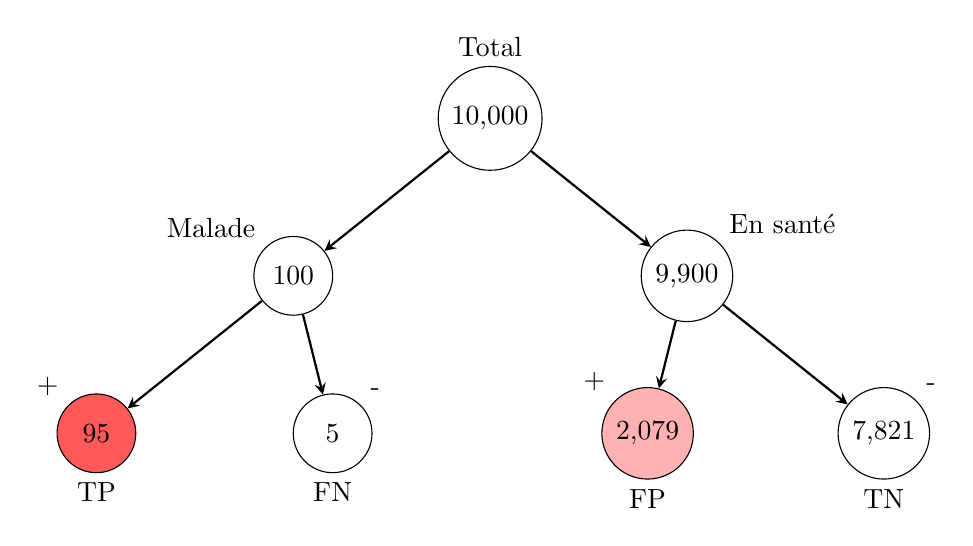
\begin{tikzpicture}
    \tikzstyle{arrow} = [thick,->,>=stealth]
    % Top bubble
    \node [draw, circle, minimum size=1cm, text centered, label={90:Total}] (Top) at (0,5) {10,000};

    % Lower left bubble
    \node [draw, circle, minimum size=1cm, text centered, label={135:Malade}] (Diseased) at (-2.5,3) {100};
    \draw [arrow] (Top) -- (Diseased);

    % Lower right bubble
    \node [draw, circle, minimum size=1cm, text centered, label={45:En santé}] (NonDiseased) at (2.5,3) {9,900};
    \draw [arrow] (Top) -- (NonDiseased);

    % Bottom extreme left
    \node [draw, circle, minimum size=1cm, text centered, label={135:+}, label={-90:TP}, fill=red!65] (TP) at (-5,1) {95};
    \draw [arrow] (Diseased) -- (TP);

    % Bottom mid left
    \node [draw, circle, minimum size=1cm, text centered, label={45:-}, label={-90:FN}] (FN) at (-2,1) {5};
    \draw [arrow] (Diseased) -- (FN);

    % Bottom mid right
    \node [draw, circle, minimum size=1cm, text centered, label={135:+}, label={-90:FP}, fill=red!30] (FP) at (2,1) {2,079};
    \draw [arrow] (NonDiseased) -- (FP);

    % Bottom extreme right
    \node [draw, circle, minimum size=1cm, text centered, label={45:-}, label={-90:TN}] (TN) at (5,1) {7,821};
    \draw [arrow] (NonDiseased) -- (TN);
\end{tikzpicture}

